
\section{Simulations}


\begin{table}[H]
    \begin{center}
        \caption{Size of the test calculated for different sample sizes ($T = 250, 350, 500, 1000$) and confident levels ($\alpha = 0.01, 0.05, 0.10$)}
        \label{tab:size_nw}
        \centering
        % latex table generated in R 3.4.3 by xtable 1.8-2 package
% 
\begin{tabular}{rrrr}
  \hline
 & 0.01 & 0.05 & 0.1 \\ 
  \hline
250 & 0.007 & 0.033 & 0.072 \\ 
  350 & 0.005 & 0.041 & 0.087 \\ 
  500 & 0.015 & 0.054 & 0.078 \\ 
   \hline
\end{tabular}

    \end{center}
\end{table}

\begin{table}[H]
    \begin{center}
        \caption{Power of the test calculated for different sample sizes ($T = 250, 350, 500, 1000$) and confident levels ($\alpha = 0.01, 0.05, 0.10$) for $a = 0.25$}
        \label{tab:power_025_nw}
        \centering
        % latex table generated in R 3.4.3 by xtable 1.8-2 package
% 
\begin{tabular}{rrrr}
  \hline
 & 0.01 & 0.05 & 0.1 \\ 
  \hline
250 & 0.032 & 0.092 & 0.155 \\ 
  350 & 0.018 & 0.090 & 0.199 \\ 
  500 & 0.069 & 0.169 & 0.212 \\ 
   \hline
\end{tabular}

    \end{center}
\end{table}

\begin{table}[H]
    \begin{center}
        \caption{Power of the test calculated for different sample sizes ($T = 250, 350, 500, 1000$) and confident levels ($\alpha = 0.01, 0.05, 0.10$) for $a = 0.50$}
        \label{tab:power_050_nw}
        \centering
        % latex table generated in R 3.4.3 by xtable 1.8-2 package
% 
\begin{tabular}{rrrr}
  \hline
 & 0.01 & 0.05 & 0.1 \\ 
  \hline
250 & 0.153 & 0.265 & 0.399 \\ 
  350 & 0.192 & 0.333 & 0.517 \\ 
  500 & 0.355 & 0.571 & 0.694 \\ 
   \hline
\end{tabular}

    \end{center}
\end{table}

\begin{table}[H]
    \begin{center}
        \caption{Power of the test calculated for different sample sizes ($T = 250, 350, 500, 1000$) and confident levels ($\alpha = 0.01, 0.05, 0.10$) for $a = 0.65$}
        \label{tab:power_065_nw}
        \centering
        % latex table generated in R 3.4.3 by xtable 1.8-2 package
% 
\begin{tabular}{rrrr}
  \hline
 & 0.01 & 0.05 & 0.1 \\ 
  \hline
250 & 0.321 & 0.471 & 0.590 \\ 
  350 & 0.416 & 0.620 & 0.744 \\ 
  500 & 0.686 & 0.846 & 0.900 \\ 
   \hline
\end{tabular}

    \end{center}
\end{table}

\begin{table}[H]
    \begin{center}
        \caption{Power of the test calculated for different sample sizes ($T = 250, 350, 500, 1000$) and confident levels ($\alpha = 0.01, 0.05, 0.10$) for $a = 0.75$}
        \label{tab:power_075_nw}
        \centering
        % latex table generated in R 3.4.3 by xtable 1.8-2 package
% 
\begin{tabular}{rrrr}
  \hline
 & 0.01 & 0.05 & 0.1 \\ 
  \hline
250 & 0.461 & 0.625 & 0.754 \\ 
  350 & 0.571 & 0.793 & 0.888 \\ 
  500 & 0.862 & 0.936 & 0.968 \\ 
   \hline
\end{tabular}

    \end{center}
\end{table}

\begin{table}[H]
    \begin{center}
        \caption{Power of the test calculated for different sample sizes ($T = 250, 350, 500, 1000$) and confident levels ($\alpha = 0.01, 0.05, 0.10$) for $a = 1.0$}
        \label{tab:power_100_nw}
        \centering
        % latex table generated in R 3.4.3 by xtable 1.8-2 package
% 
\begin{tabular}{rrrr}
  \hline
 & 0.01 & 0.05 & 0.1 \\ 
  \hline
250 & 0.760 & 0.913 & 0.943 \\ 
  350 & 0.918 & 0.968 & 0.986 \\ 
  500 & 0.992 & 1.000 & 1.000 \\ 
   \hline
\end{tabular}

    \end{center}
\end{table}



\newpage
\section{Data analysis}


\begin{figure}[ht!]
\centering
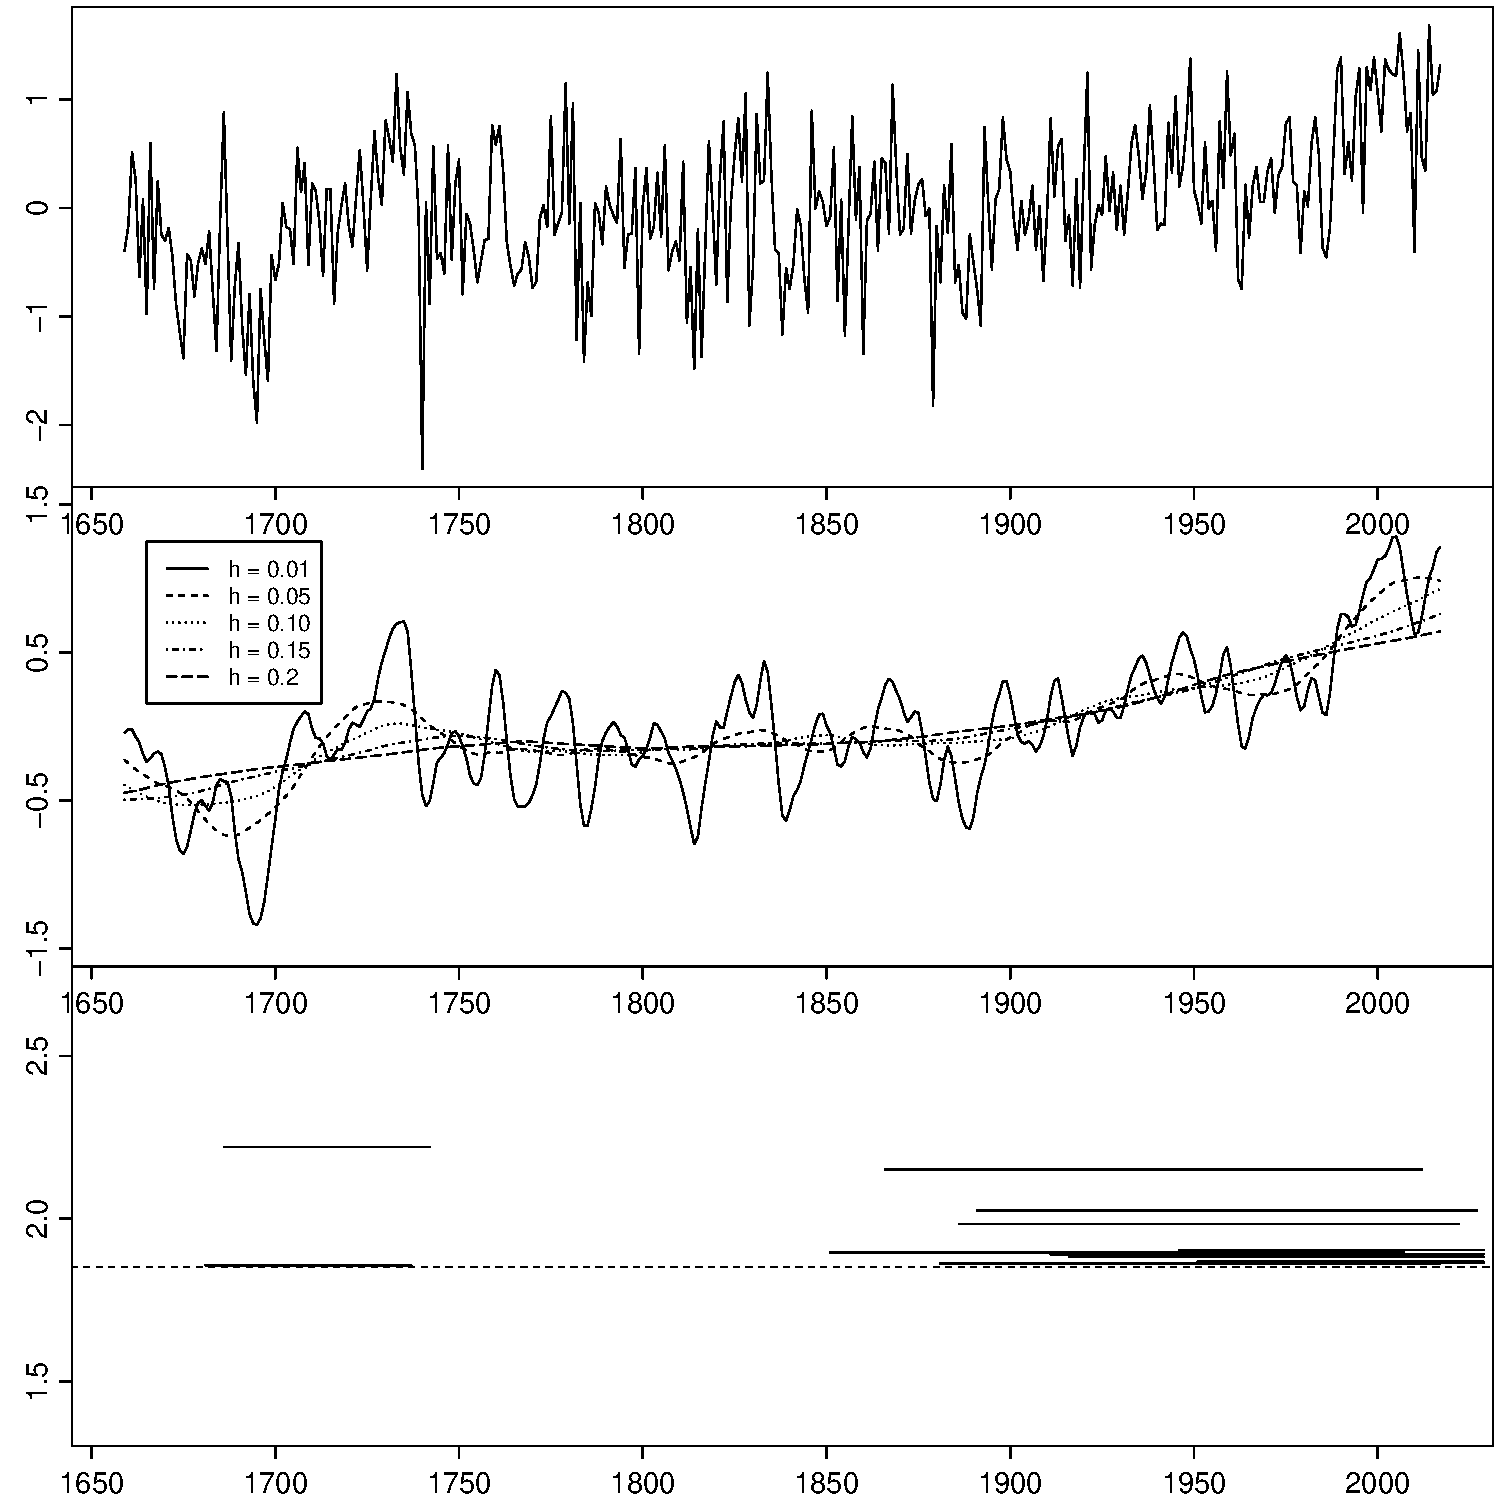
\includepdf[pages=-,pagecommand={},width=\textwidth]{Coding/Output/threegraphics_testing_constant_method_ll.pdf}
\caption{Yearly temperature data for England\label{yearly_data}}
\end{figure}

